% =============================================================================
% slides.tex -- Data Analytics semestral project, topic: Specialty Cafes
% Uses the figures and the number macros written by analysis/03_analysis.R.
% Compile from the presentation/ folder:  latexmk -pdf slides.tex
% =============================================================================
\documentclass[aspectratio=169,11pt]{beamer}
\usetheme{default}
\usecolortheme{dove}
\setbeamertemplate{navigation symbols}{}
\setbeamertemplate{footline}[frame number]
\setbeamerfont{frametitle}{series=\bfseries}
\usepackage[T1]{fontenc}
\usepackage{booktabs}
\usepackage{adjustbox}
\graphicspath{{../report/figures/}}

\newcommand{\meanci}[4]{$M = #1$\,#4, 95\%~CI [#2, #3]}
\newcommand{\mdiffci}[4]{$M_\Delta = #1$\,#4, 95\%~CI [#2, #3]}
\newcommand{\diffci}[7]{$M_\Delta = #1$\,#4, 95\%~CI [#2, #3], $d = #5$, 95\%~CI [#6, #7]}
\newcommand{\dci}[3]{$d = #1$, 95\%~CI [#2, #3]}
\newcommand{\tstat}[2]{$t(#1) = #2$}
\newcommand{\pval}[1]{$p = #1$}
\newcommand{\plt}[1]{$p < #1$}
\newcommand{\Fstat}[3]{$F(#1, #2) = #3$}
% Written by analysis/03_analysis.R -- do not edit by hand.
\newcommand{\BenchCZK}{86.58}
\newcommand{\USDCZK}{21.646}
\newcommand{\Nall}{189}
\newcommand{\Nfilter}{54}
\newcommand{\Boot}{5,000}
\newcommand{\Seed}{2026}
\newcommand{\AoneN}{54}
\newcommand{\AoneEst}{\meanci{84.5}{80.3}{88.7}{CZK}}
\newcommand{\AoneDiff}{\mdiffci{\ensuremath{-}2.1}{\ensuremath{-}6.3}{2.1}{CZK}}
\newcommand{\AoneD}{\dci{\ensuremath{-}0.14}{\ensuremath{-}0.40}{0.13}}
\newcommand{\AoneT}{\tstat{53}{\ensuremath{-}1.00}, \pval{.321}}
\newcommand{\AoneMedian}{85.0}
\newcommand{\AoneWil}{$V = 590$, \pval{.190}}
\newcommand{\AoneBoot}{84.5 [80.6, 88.6]}
\newcommand{\AtwoNone}{54}
\newcommand{\AtwoNzero}{133}
\newcommand{\AtwoMone}{67.4}
\newcommand{\AtwoMzero}{63.5}
\newcommand{\AtwoEst}{\diffci{3.9}{0.1}{7.7}{CZK}{0.32}{0.00}{0.63}}
\newcommand{\AtwoT}{\tstat{105.5}{2.02}, \pval{.023} (one-tailed)}
\newcommand{\AtwoLower}{0.7}
\newcommand{\AtwoWil}{$W = 4370$, \pval{.010} (one-tailed)}
\newcommand{\AtwoHL}{5.0 [0.0, 7.0]}
\newcommand{\AtwoBoot}{3.9 [0.2, 7.6]}
\newcommand{\AtwoLevene}{\Fstat{1}{185}{0.17}, \pval{.682}}
\newcommand{\AthreeN}{54}
\newcommand{\AthreeEst}{\meanci{17.1}{13.9}{20.4}{CZK}}
\newcommand{\AthreeDz}{$d_z = 1.45$, 95\% CI [1.06, 1.83]}
\newcommand{\AthreeT}{\tstat{53}{10.65}, \plt{.001} (one-tailed)}
\newcommand{\AthreeMedian}{15.0}
\newcommand{\AthreeZero}{2}
\newcommand{\AthreeMax}{75}
\newcommand{\AthreeTrim}{16.0 [13.6, 18.5]}
\newcommand{\AthreeWil}{$V = 1378$, \plt{.001} (one-tailed)}
\newcommand{\AthreeBoot}{17.1 [14.3, 20.3]}
\newcommand{\AfourN}{187}
\newcommand{\AfourMNone}{\meanci{63.5}{61.2}{65.8}{CZK}}
\newcommand{\AfourNNone}{125}
\newcommand{\AfourMOne}{\meanci{66.2}{63.0}{69.5}{CZK}}
\newcommand{\AfourNOne}{49}
\newcommand{\AfourMBoth}{\meanci{69.3}{62.6}{76.0}{CZK}}
\newcommand{\AfourNBoth}{13}
\newcommand{\AfourF}{\Fstat{2}{33.1}{2.12}, \pval{.136}}
\newcommand{\AfourEta}{$\eta^2 = 0.020$, 95\% CI [0.000, 0.069]}
\newcommand{\AfourClassic}{\Fstat{2}{184}{1.89}, \pval{.153}}
\newcommand{\AfourLevene}{\Fstat{2}{184}{0.74}, \pval{.476}}
\newcommand{\AfourKW}{$H(2) = 6.42$, \pval{.040}}
\newcommand{\AfourGHOneNone}{$M_\Delta = 2.8$~CZK, 95\% CI [\ensuremath{-}1.9, 7.5], $p_{\text{adj}} = .339$}
\newcommand{\AfourGHBothNone}{$M_\Delta = 5.8$~CZK, 95\% CI [\ensuremath{-}2.6, 14.3], $p_{\text{adj}} = .206$}
\newcommand{\AfourGHBothOne}{$M_\Delta = 3.1$~CZK, 95\% CI [\ensuremath{-}5.7, 11.8], $p_{\text{adj}} = .654$}
\newcommand{\AfiveN}{187}
\newcommand{\AfiveRoast}{13 of 21 (61.9\%)}
\newcommand{\AfiveOther}{41 of 166 (24.7\%)}
\newcommand{\AfivePP}{37.2 percentage points, 95\% CI [15.4, 59.0]}
\newcommand{\AfiveChi}{$\chi^2(1, N = 187) = 12.56$, \plt{.001}}
\newcommand{\AfiveMinExp}{6.1}
\newcommand{\AfiveV}{$V = 0.26$, 95\% CI [0.09, 0.41]}
\newcommand{\AfiveRes}{3.54}
\newcommand{\AfiveFisher}{$\text{OR} = 4.90$, 95\% CI [1.74, 14.69], \pval{.001}}
\newcommand{\AsixN}{54}
\newcommand{\AsixR}{$r = 0.64$, 95\% CI [0.46, 0.78]}
\newcommand{\AsixT}{\tstat{52}{6.08}, \plt{.001}}
\newcommand{\AsixRho}{$\rho = 0.73$, 95\% CI [0.56, 0.85], \plt{.001}}
\newcommand{\AsixTau}{$\tau = 0.60$, 95\% CI [0.45, 0.74], \plt{.001}}
\newcommand{\AsixBoot}{[0.48, 0.83]}
\newcommand{\AsixRsq}{0.42}
\newcommand{\AsevenN}{54}
\newcommand{\AsevenB}{$b = 8.42$~CZK per 10~CZK, robust 95\% CI [6.20, 10.65]}
\newcommand{\AsevenT}{\tstat{52}{7.60}, \plt{.001}}
\newcommand{\AsevenRsq}{0.416}
\newcommand{\AsevenInt}{27.7}
\newcommand{\AsevenClassic}{[5.65, 11.20]}
\newcommand{\AsevenBoot}{[6.47, 10.97]}
\newcommand{\AsevenInfl}{3}
\newcommand{\AsevenNoInfl}{$b = 8.01$, 95\% CI [6.01, 10.02]}
\newcommand{\AeightN}{187}
\newcommand{\AeightBone}{$b = 3.90$~CZK, robust 95\% CI [0.06, 7.74], \pval{.047}}
\newcommand{\AeightBtwo}{$b = 4.40$~CZK, robust 95\% CI [0.58, 8.22], \tstat{184}{2.27}, \pval{.024}}
\newcommand{\AeightDist}{$b = \ensuremath{-}1.73$~CZK per km, robust 95\% CI [\ensuremath{-}3.02, \ensuremath{-}0.44], \pval{.009}}
\newcommand{\AeightChange}{0.50}
\newcommand{\AeightChangePct}{13}
\newcommand{\AeightF}{\Fstat{1}{184}{6.53}, \pval{.011}}
\newcommand{\AeightFrob}{\Fstat{1}{184}{6.99}, \pval{.009}}
\newcommand{\AeightVIF}{1.01}
\newcommand{\AeightRsqOne}{0.020}
\newcommand{\AeightRsqTwo}{0.054}
\newcommand{\AeightLog}{$b = 4.65$, 95\% CI [0.89, 8.41]}
\newcommand{\AeightInfl}{10}
\newcommand{\AeightNoInfl}{$b = 4.12$, 95\% CI [0.87, 7.36]}
\newcommand{\AnineN}{54}
\newcommand{\AnineNind}{35}
\newcommand{\AnineNchain}{19}
\newcommand{\AnineB}{$b = \ensuremath{-}6.02$~CZK per 10~CZK, robust 95\% CI [\ensuremath{-}12.00, \ensuremath{-}0.05], \tstat{50}{\ensuremath{-}2.02}, \pval{.048}}
\newcommand{\AnineF}{\Fstat{1}{50}{4.00}, \pval{.051}}
\newcommand{\AnineFrob}{\Fstat{1}{50}{4.10}, \pval{.048}}
\newcommand{\AnineSind}{$b = 11.44$~CZK, 95\% CI [6.22, 16.65]}
\newcommand{\AnineSchain}{$b = 5.41$~CZK, 95\% CI [2.48, 8.34]}
\newcommand{\AnineRsq}{0.459}
\newcommand{\AnineInfl}{3}
\newcommand{\AnineNoInfl}{$b = \ensuremath{-}7.18$, 95\% CI [\ensuremath{-}12.49, \ensuremath{-}1.86]}
\newcommand{\AnineVIF}{1.23}
\newcommand{\AtenN}{187}
\newcommand{\AtenEvents}{54}
\newcommand{\AtenAME}{4.5 percentage points per km, 95\% CI [0.9, 8.1], $z = 2.43$, \pval{.015}}
\newcommand{\AtenOR}{$\text{OR} = 1.25$ per km, 95\% CI [1.04, 1.52]}
\newcommand{\AtenBoot}{[0.9, 7.9]}
\newcommand{\AtenLPM}{4.6 percentage points, 95\% CI [0.9, 8.3]}
\newcommand{\AtenInfl}{8}
\newcommand{\AtenNoInfl}{6.3 percentage points, 95\% CI [2.4, 10.2]}
\newcommand{\AtenPwest}{17}
\newcommand{\AtenPzero}{24}
\newcommand{\AtenPeast}{44}
\newcommand{\HolmSig}{4}
\newcommand{\RawSig}{8}
\newcommand{\BPseven}{.933}
\newcommand{\BPeight}{.093}
\newcommand{\BPnine}{.538}
\newcommand{\Rversion}{4.6.1}
\newcommand{\Versandwich}{3.1.3}
\newcommand{\Verlmtest}{0.9.40}
\newcommand{\Vercar}{3.1.5}
\newcommand{\Vermarginaleffects}{1.0.0}


\title{Filter coffee in Prague caf\'es}
\subtitle{Priced close to 4 USD, about 17 CZK above an espresso, offered mostly by roasteries}
\author{Aidan Osbaugh}
\institute{Data Analytics, Batch \textit{N} \quad Partner: \textit{name}}
\date{\today}

\begin{document}

\begin{frame}
\titlepage
\end{frame}

\begin{frame}{Data and approach}
\begin{itemize}
  \item \Nall{} Prague caf\'es recorded by the class; 299 raw rows $\to$ 99 empty rows and 11 double entries removed
  \item \Nfilter{} caf\'es sell filter coffee (a price), 133 do not (``NA''), 2 unknown (blank $\to$ missing)
  \item Ten questions A1--A10, hypotheses and directions fixed in advance; $\alpha = .05$
  \item Prices are right-skewed, but every compared group is near-normal or $n \ge 49$ $\to$ parametric tests first, rank-based and bootstrap tests as checks (\Boot{} resamples, seed \Seed)
  \item Regressions with HC3 robust standard errors; logit reported as average marginal effect
\end{itemize}
\end{frame}

\begin{frame}{All ten results}
\centering\scriptsize
\begin{adjustbox}{max width=\textwidth}\begin{tabular}{lllrrlll}
\toprule
 & Question & Method & $n$ & Lost & Estimate [95\% CI] & Effect size [95\% CI] & $p$ \\
\midrule
A1 & Filter coffee price vs 4 USD & One-sample $t$ & 54 & 135 & $M = 84.5$ [80.3, 88.7] CZK & $d = \ensuremath{-}0.14$ [\ensuremath{-}0.40, 0.13] & .321 \\
A2 & Espresso: filter minus no filter & Welch $t$ (one-tailed) & 187 &   2 & $M_\Delta = 3.9$ [0.1, 7.7] CZK & $d = 0.32$ [0.00, 0.63] & .023 \\
A3 & Filter minus espresso, same caf\'e & Paired $t$ (one-tailed) & 54 & 135 & $M_d = 17.1$ [13.9, 20.4] CZK & $d_z = 1.45$ [1.06, 1.83] & < .001 \\
A4 & Espresso by specialty features & Welch ANOVA & 187 &   2 & Both $-$ None: 5.8 [\ensuremath{-}2.6, 14.3] CZK & $\eta^2 = 0.020$ [0.000, 0.069] & .136 \\
A5 & Roastery $\times$ offers filter & $\chi^2$ test & 187 &   2 & 37.2 pp [15.4, 59.0] & $V = 0.26$ [0.09, 0.41] & < .001 \\
A6 & Filter and espresso price & Pearson $r$ & 54 & 135 & $r = 0.64$ [0.46, 0.78] & $\rho = 0.73$ & < .001 \\
A7 & Filter price per 10 CZK espresso & OLS, HC3 SE & 54 & 135 & $b = 8.42$ [6.20, 10.65] CZK & $R^2 = 0.416$ & < .001 \\
A8 & Filter gap, adjusted for distance & OLS, HC3 SE & 187 &   2 & $b = 4.40$ [0.58, 8.22] CZK & $R^2 = 0.054$ & .024 \\
A9 & Espresso slope: chain vs independent & OLS interaction, HC3 & 54 & 135 & $b_{\times} = \ensuremath{-}6.02$ [\ensuremath{-}12.00, \ensuremath{-}0.05] CZK & $R^2 = 0.459$ & .048 \\
A10 & Offers filter, per km east & Logit, AME & 187 &   2 & 4.5 pp [0.9, 8.1] & OR $= 1.25$ [1.04, 1.52] & .015 \\
\bottomrule
\end{tabular}
\end{adjustbox}

\vspace{0.6em}
\small Holm adjustment across the ten tests: \HolmSig{} of \RawSig{} significant results remain (A3, A5, A6, A7).
\end{frame}

\begin{frame}{A1 \& A3: What a filter coffee costs}
\begin{columns}[T]
\column{0.5\textwidth}
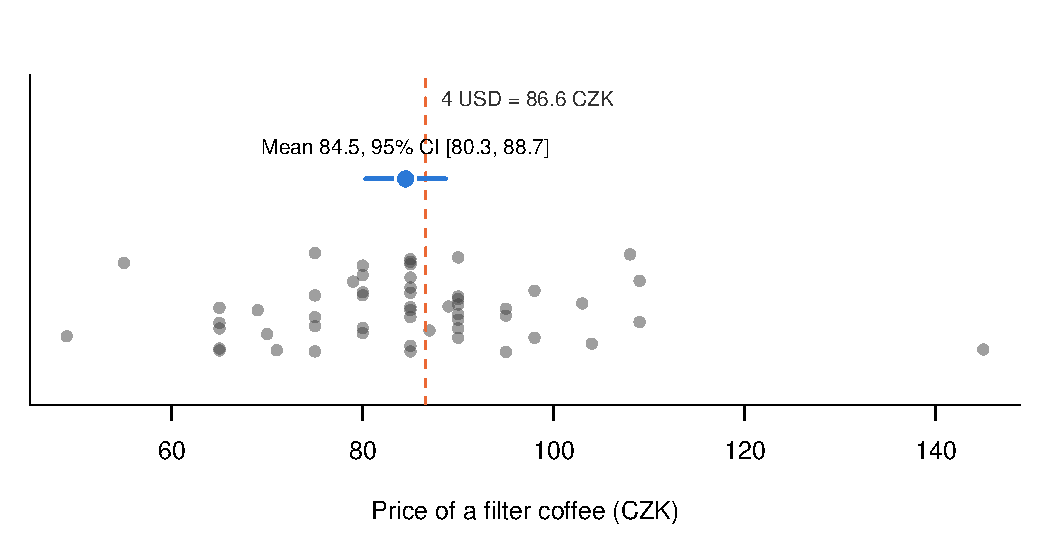
\includegraphics[width=\linewidth]{A1_figure.pdf}\\[0.3em]
\small\textbf{A1} \AoneEst; vs 4 USD (\BenchCZK\,CZK): \AoneT{} $\to$ \emph{no detectable difference}
\column{0.5\textwidth}
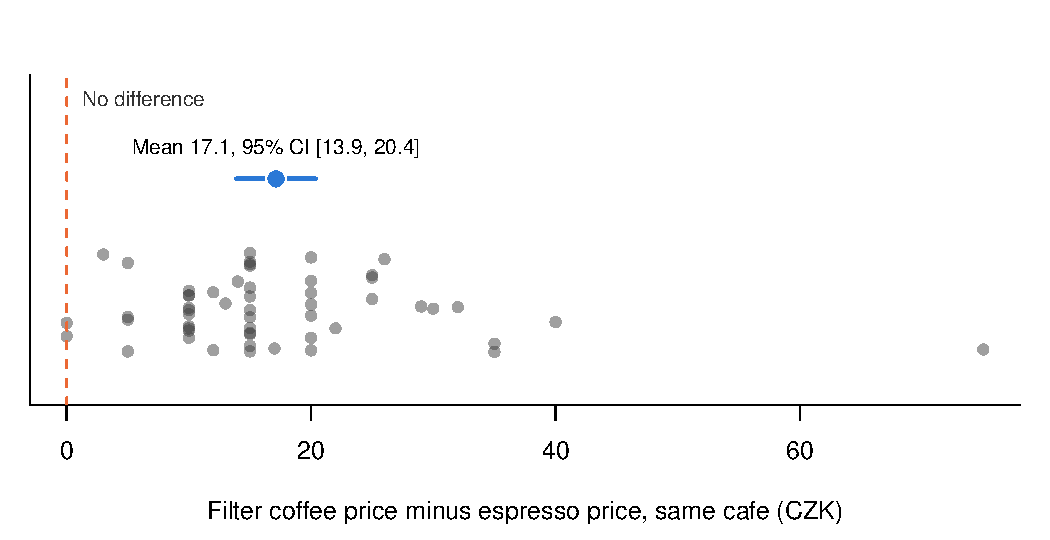
\includegraphics[width=\linewidth]{A3_figure.pdf}\\[0.3em]
\small\textbf{A3} Filter $-$ espresso, same caf\'e: \AthreeEst, \AthreeDz{} $\to$ \emph{about 17 CZK more}
\end{columns}
\end{frame}

\begin{frame}{A5: Roasteries offer filter coffee far more often}
\begin{columns}[c]
\column{0.45\textwidth}
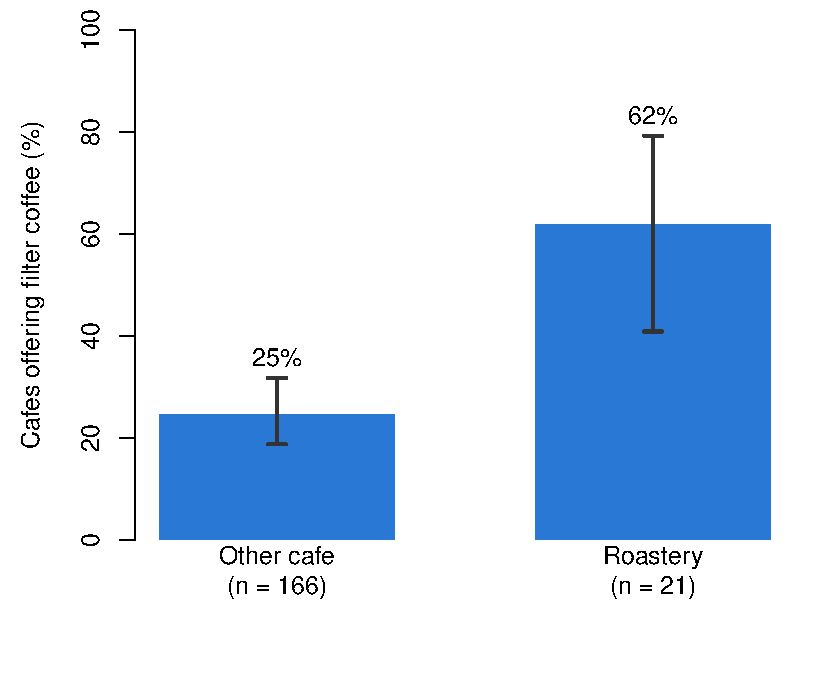
\includegraphics[width=\linewidth]{A5_figure.pdf}
\column{0.55\textwidth}
\begin{itemize}
  \item Roasteries: \AfiveRoast
  \item Other caf\'es: \AfiveOther
  \item Difference: \AfivePP
  \item \AfiveChi; \AfiveV
\end{itemize}
\end{columns}
\end{frame}

\begin{frame}{A6 \& A7: Filter prices track espresso prices}
\begin{columns}[c]
\column{0.45\textwidth}
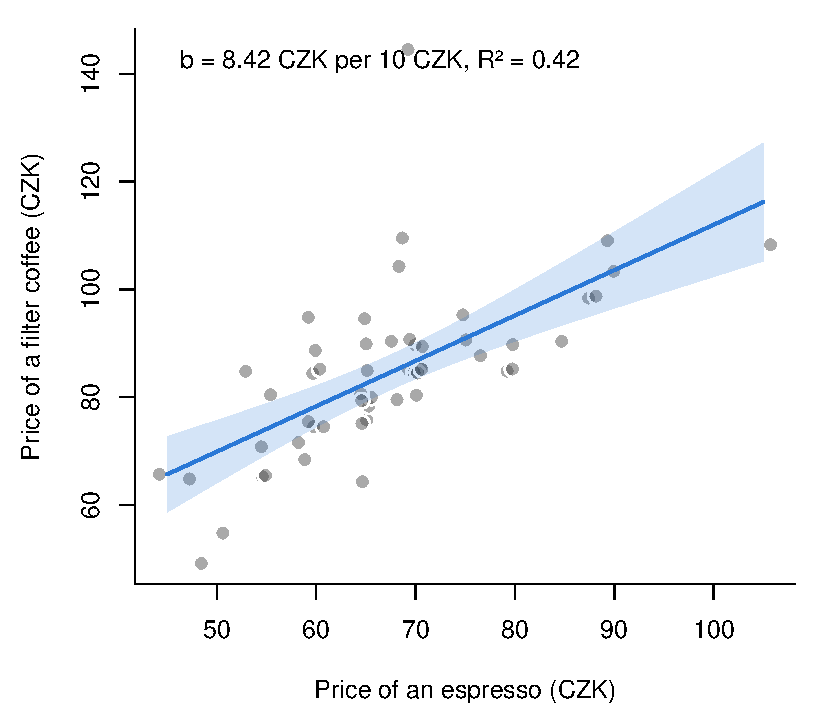
\includegraphics[width=\linewidth]{A7_figure.pdf}
\column{0.55\textwidth}
\begin{itemize}
  \item \AsixR{} (Spearman $\rho = 0.73$)
  \item \AsevenB
  \item $R^2 = \AsevenRsq$; residuals well-behaved; holds without influential caf\'es
  \item Association only --- nothing about causes
\end{itemize}
\end{columns}
\end{frame}

\begin{frame}{A2 \& A8: Espresso costs a little more where filter is offered}
\begin{columns}[c]
\column{0.5\textwidth}
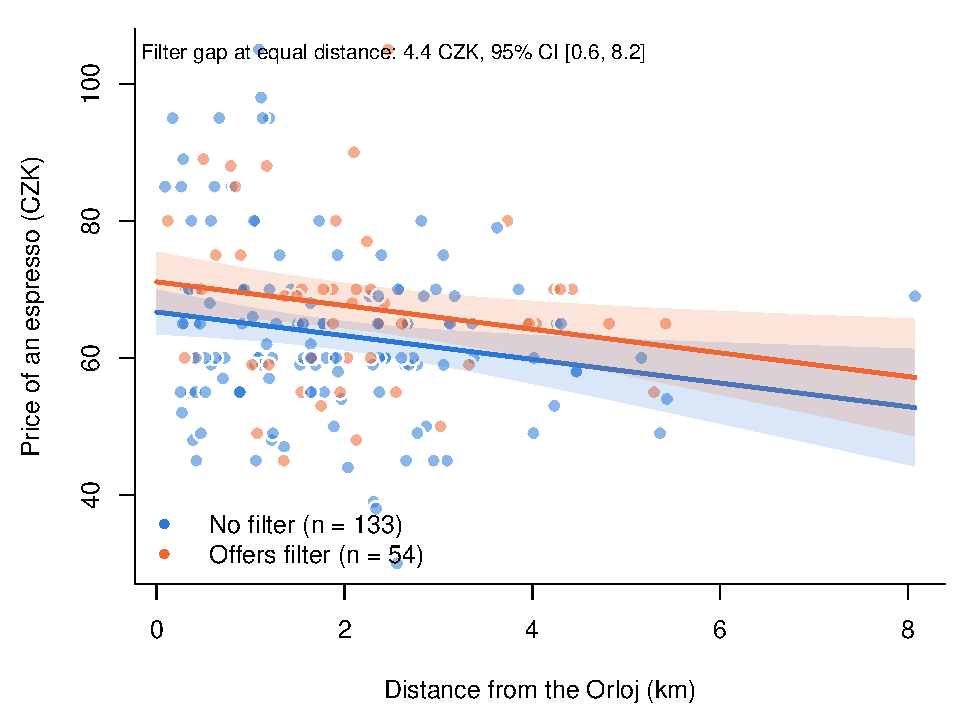
\includegraphics[width=\linewidth]{A8_figure.pdf}
\column{0.5\textwidth}
\begin{itemize}
  \item A2: \AtwoEst; \AtwoT
  \item A8, adjusted for distance from the Orloj: \AeightBtwo
  \item Espresso is cheaper further out: \AeightDist
  \item Small effects; not significant after Holm adjustment
\end{itemize}
\end{columns}
\end{frame}

\begin{frame}{A4 \& A9: Weak or borderline}
\begin{columns}[T]
\column{0.5\textwidth}
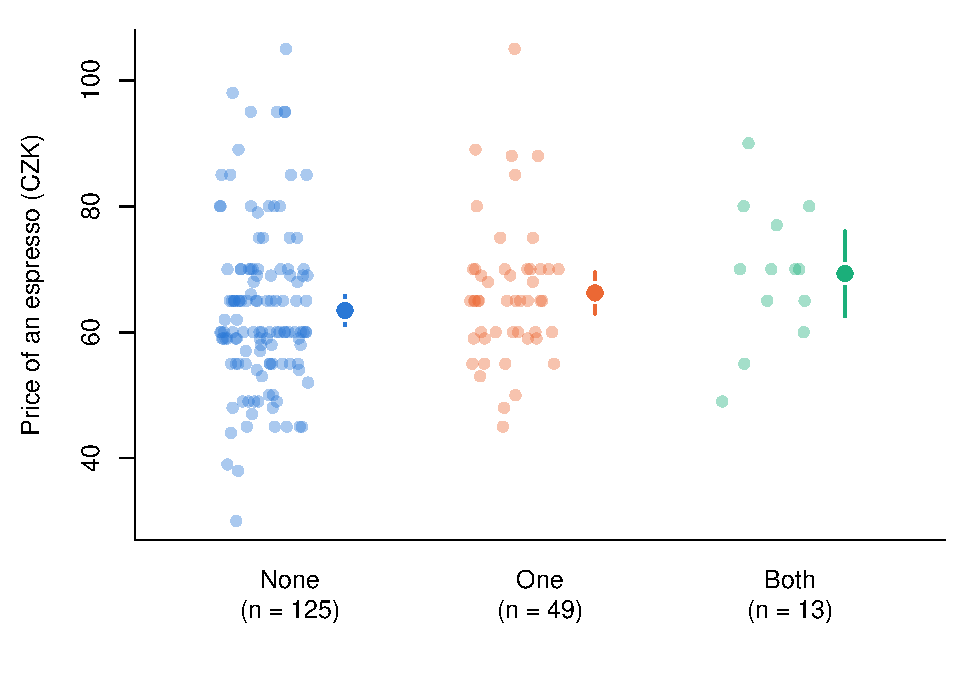
\includegraphics[width=\linewidth]{A4_figure.pdf}\\[0.2em]
\scriptsize\textbf{A4} \AfourF, \AfourEta; Kruskal--Wallis \AfourKW{} $\to$ \emph{inconclusive}
\column{0.5\textwidth}
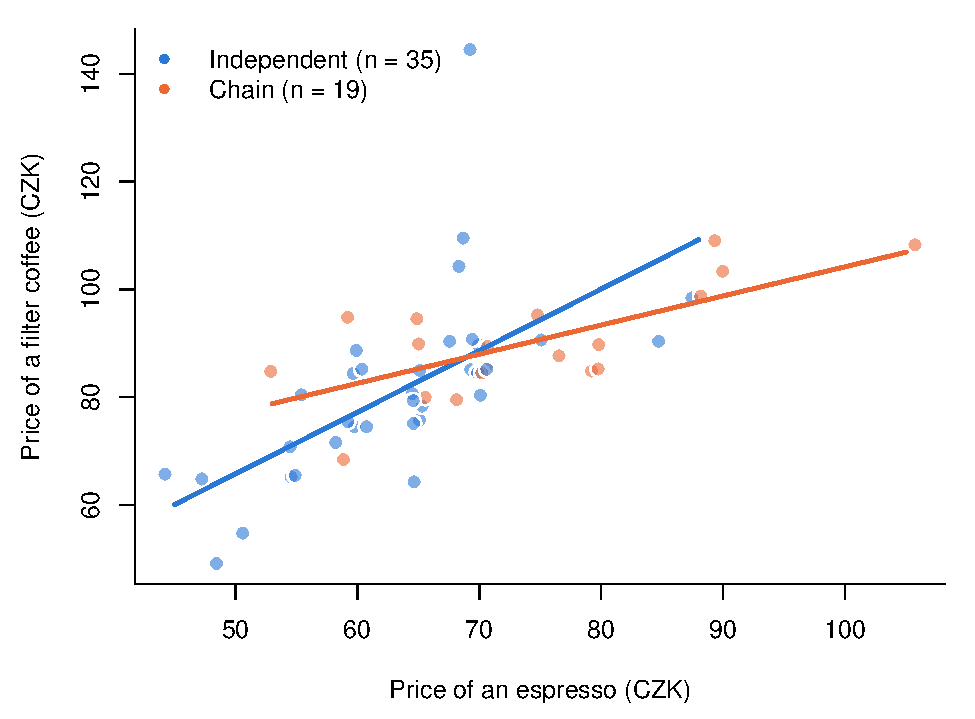
\includegraphics[width=\linewidth]{A9_figure.pdf}\\[0.2em]
\scriptsize\textbf{A9} Slope independent \AnineSind{} vs chains \AnineSchain; interaction $p = .048$ (classic $F$: $p = .051$) $\to$ \emph{borderline}
\end{columns}
\end{frame}

\begin{frame}{A10: Filter coffee is more common east of the Orloj}
\begin{columns}[c]
\column{0.5\textwidth}
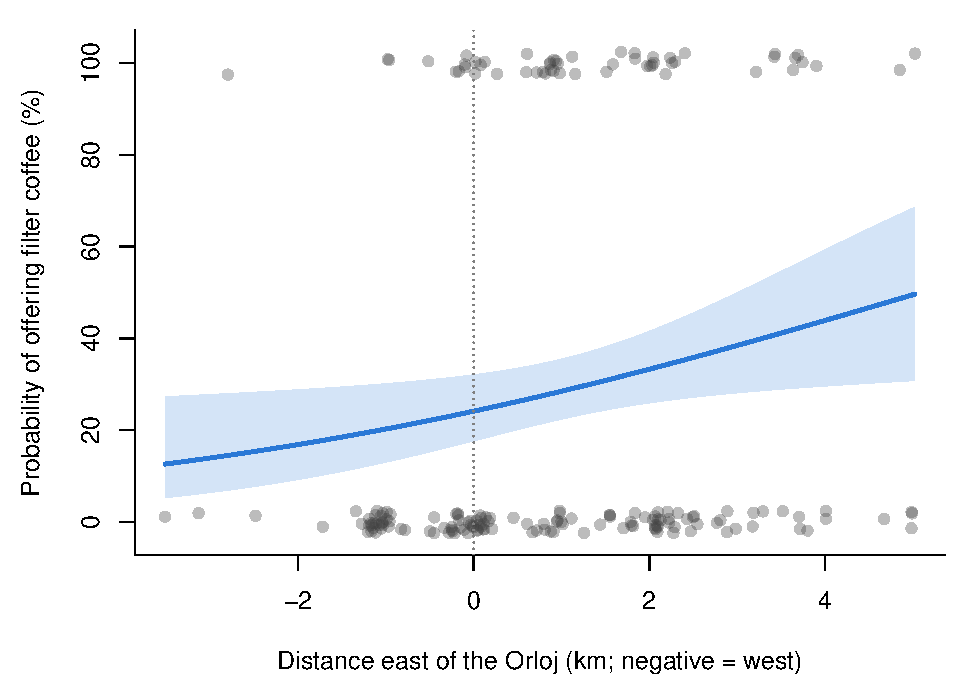
\includegraphics[width=\linewidth]{A10_figure.pdf}
\column{0.5\textwidth}
\begin{itemize}
  \item Average marginal effect: \AtenAME
  \item Predicted: \AtenPwest\% at 2 km west, \AtenPzero\% at the Orloj, \AtenPeast\% at 4 km east
  \item Check: \AtenOR
  \item $n = \AtenN$, \AtenEvents{} caf\'es with filter coffee
\end{itemize}
\end{columns}
\end{frame}

\begin{frame}{Conclusions and limits}
\begin{itemize}
  \item \textbf{Robust:} filter coffee costs about 4 USD, about 17 CZK more than an espresso, tracks the espresso price, and is concentrated in roasteries
  \item \textbf{Exploratory:} the 4 CZK espresso premium (A2, A8), the steeper price link in independents (A9), more filter coffee to the east (A10)
  \item \textbf{Limits:} convenience sample collected by students; observational data; caf\'es in the same district are not independent; only 54 caf\'es with filter coffee and 19 chains among them
  \item All claims hold \emph{in this sample}
\end{itemize}
\vspace{0.5em}
\scriptsize Code and data: \url{https://github.com/aidanosbaugh/data-analytics-semestral-project}
\end{frame}

\end{document}
